\section{Makaron z łososiem i warzywami*}
\bigskip
\small
\begin{minipage}{0.45\textwidth}
    \noindent \textbf{Czas:} 20 minut \\
    \textbf{Poziom trudności:} umiarkowany
\end{minipage}
\begin{minipage}{0.45\textwidth}
    \noindent \textbf{Ilość sprzątania:} średnia\\
    \textbf{Wymagany mysi sprzęt:} -
\end{minipage}
\normalsize
\vspace{0.5cm}

\begin{multicols}{2}

\subsection*{Składniki} \begin{itemize}
    \item 50-100 g wędzonego łososia
    \item 2 ząbki czosnku
    \item porcja makaronu
    \item 2 garści młodego szpinaku
    \item garść pomidorków koktajlowych
    \item 50 g śmietanki 18\%
    \item oliwa do smażenia
    \item sól i pieprz do smaku
\end{itemize}

\columnbreak

\begin{figure}[H]
    \centering
    \fbox{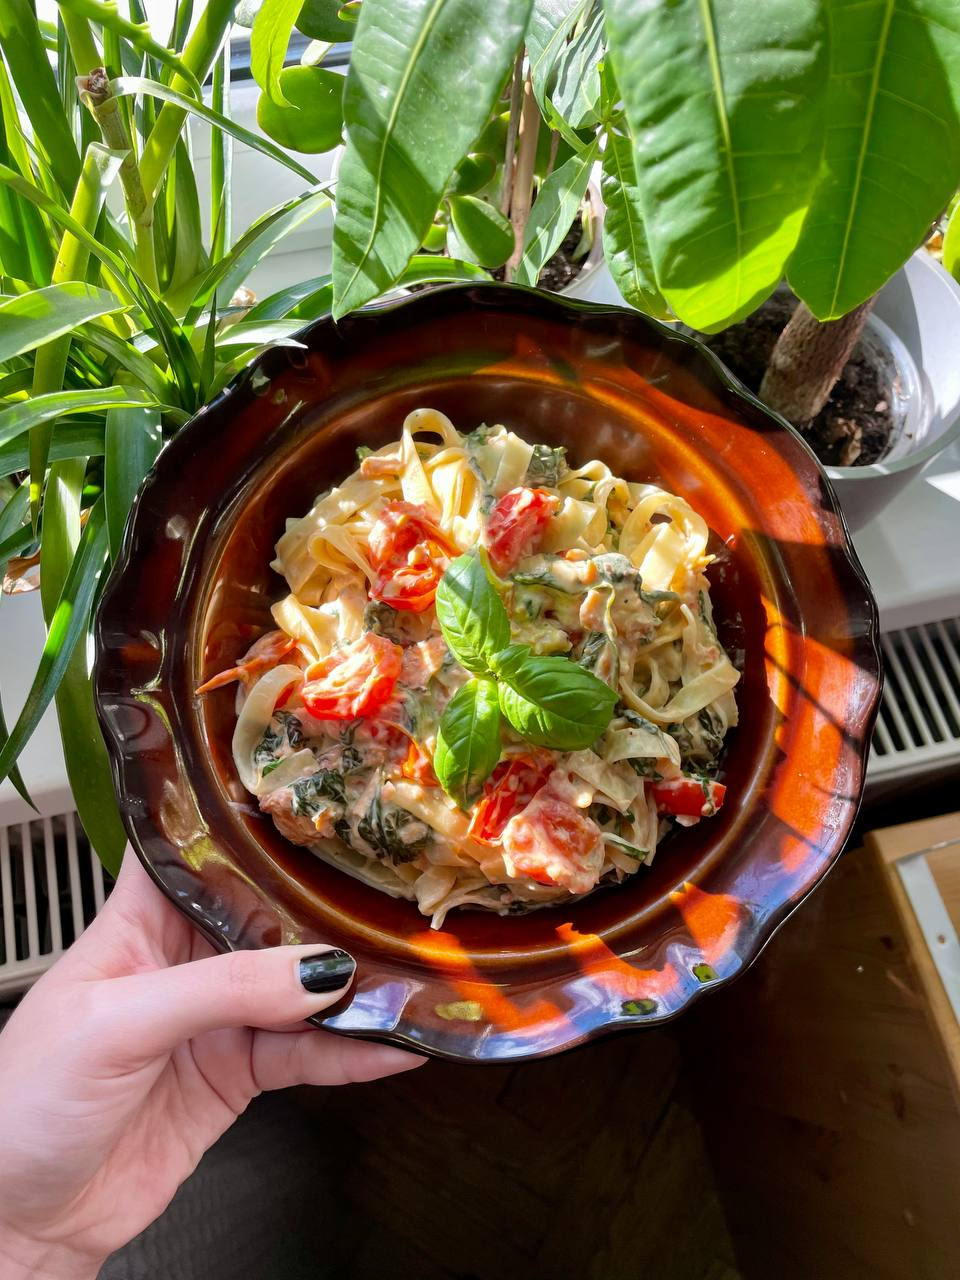
\includegraphics[width=0.35\textwidth]{images/makaron-z-lososiem.jpg}}
\end{figure}
\end{multicols}

\vspace{0.5cm}

\subsection*{Instruktaż}
\begin{enumerate}
    \item Pomidorki przekrojone w pól podsmażać na dobrze rozgrzanej patelni wraz ze szczyptą soli przez ok. 3 minuty, lub do momentu, aż się zarumienią. Dosypać szpinak i smażyć aż wytraci całą wodę.
    \item Szpinak i pomidorki odsunąć na bok patelni, zmniejszyć moc palnika i na patelni podsmażyć wędzonego łososia poszarpanego na niewielkie kawałki przez ok. 3 minuty. Wszystko dokładnie wymieszać i na boku patelni delikatnie podsmażyć przeciśnięty przez praskę czosnek przez ok. 30 sekund. Całość zalać śmietanką, wymieszać i zagotować. Po zagotowaniu zmniejszyć na minimalny ogień i delikatnie dusić pod przykrywką przez ok. 10 minut, od czasu do czasu mieszając.
    \item W międzyczasie ugotować makaron zgodnie z instrukcją na opakowaniu i odcedzić. Ugotowany makaron przełożyć na patelnię z sosem, dokładnie wymieszać i doprawić odrobiną soli i pieprzu (uwaga na sól - wędzony łosoś jest zazwyczaj dość słony).
\end{enumerate}

\vspace{0.5cm}

\small
\subsection*{Propozycja podania} Ze startym serem, z listkami świeżej bazylii.

\vspace{0.3cm}

\subsection*{Dodatkowe uwagi} Szpinak i pomidorki można zastąpić innymi warzywami, również mrożonymi, np. brokułem, groszkiem, papryką, itp.

\newpage
